\documentclass[11pt,a4paper]{article}

% ---- Packages ----
\usepackage[utf8]{inputenc}
\usepackage[T1]{fontenc}
\usepackage{lmodern}
\usepackage[margin=1in]{geometry}
\usepackage{amsmath,amssymb}
\usepackage{graphicx}
\usepackage{booktabs}
\usepackage{hyperref}
\usepackage{cleveref}
\usepackage{enumitem}
\usepackage{xcolor}
\usepackage{listings}
\usepackage{natbib}
\usepackage{tikz}
\usepackage{multirow}
\usepackage{subcaption}

\usetikzlibrary{shapes.geometric, arrows.meta, positioning, fit, backgrounds}

\bibliographystyle{plainnat}

\hypersetup{
    colorlinks=true,
    linkcolor=blue!70!black,
    citecolor=blue!70!black,
    urlcolor=blue!70!black
}

\lstset{
    basicstyle=\ttfamily\small,
    breaklines=true,
    frame=single,
    backgroundcolor=\color{gray!8},
    keywordstyle=\color{blue!70!black},
    commentstyle=\color{green!50!black},
    stringstyle=\color{red!60!black},
}

% ---- Title ----
\title{%
\textbf{PandaEval: A Self-Evolving Framework\\for Evaluating and Improving AI Agent Skills}
}

\author{
Ji Wang\thanks{Correspondence: \texttt{jensen@srp.one}} \quad
Xiaopu Li \quad
Wenhao Xu \quad
Ning Hu \\[4pt]
Serendipity One Inc. \\
\texttt{\{jensen, sharplee, chris, felix\}@srp.one}
}

\date{March 2026}

% ================================================================
\begin{document}
\maketitle

% ---- Abstract ----
\begin{abstract}
AI agents increasingly rely on modular \emph{skills}---instruction packages that extend agent capabilities with domain-specific workflows, tool-use patterns, and output conventions.
But do these skills actually help? And can the system that evaluates them \emph{get better at evaluating them over time}?
We present \textbf{PandaEval}, a \emph{self-evolving} evaluation engine built on two interlocking feedback loops: an \textbf{evaluation loop} that blind-tests skills and accumulates grading knowledge, and an \textbf{improvement loop} that automatically rewrites underperforming skills and learns which rewrite strategies work.
We evaluate \textbf{123 real skills} from the ClawHub marketplace using Claude Opus, running each task twice---with and without the skill---and grading against deterministic assertions and LLM-as-judge rubrics.
Key findings: (1)~76.4\% of skills measurably improve model output; (2)~the evaluation engine evolved from 7 phases to 12 phases across four versions, with each version catching failure modes the previous one missed---later batches discovered \emph{assertion-skill mismatch} and \emph{framework inflation} that v0.1.0 was blind to; (3)~the improvement engine successfully upgraded 3/3 targeted skills by +1.5--2.0 points using a learned pattern library, with the counterintuitive finding that \emph{removing} 60--80\% of skill content outperforms adding to it; (4)~the system accumulated a self-evolving knowledge base of 8~failure modes, 15+~lessons, 5~improvement patterns, and 19~skill profiles, each feeding back into the methodology that produced them.
Both loops are closed: evaluation knowledge improves future evaluations, and improvement knowledge improves future improvements. The engine, like the skills it evaluates, gets measurably better over time.
All artifacts are publicly available.\footnote{\url{https://github.com/SerendipityOneInc/PandaEval}}
\end{abstract}

\noindent\textbf{Keywords:} AI agents, skill evaluation, self-evolving systems, blind A/B testing, automated improvement, benchmark

% ================================================================
\section{Introduction}
\label{sec:intro}

The shift from monolithic language models to \emph{agentic} systems---AI agents equipped with tools, permissions, and modular skills---has created a new quality assurance problem. Platforms like OpenClaw\footnote{\url{https://openclaw.ai}} and its skill marketplace ClawHub host a growing ecosystem of community-contributed skills that extend agent capabilities across domains from calendar management to financial analysis. As of March 2026, ClawHub lists over 100 published skills with no standardized quality signal.

This paper asks a simple question: \textbf{do these skills actually work?}

Existing evaluation paradigms are poorly suited to answer it. Pairwise preference arenas \citep{chiang2024chatbot} compare free-form text outputs, but skills produce \emph{actions} (creating files, calling APIs, generating structured artifacts). Static benchmarks \citep{hendrycks2021mmlu, chen2021humaneval} measure model capabilities, not the quality of instruction packages that guide models. Tool-use benchmarks \citep{qin2023toolllm, li2023apibank} evaluate whether models can call APIs, not whether a specific skill package improves the end result.

We built PandaEval to answer this question empirically. The core evaluation is deliberately simple: run each task twice on the same model---once with the skill loaded, once without---and compare outputs against the same assertions. What makes the system novel is that it doesn't just evaluate skills; it \emph{learns from its own evaluations} and \emph{learns from its own improvements}, creating two interlocking self-evolving loops.

Over five days, we evaluated 123 skills across 10 batches. The evaluation engine evolved from a basic 7-phase A/B framework (v0.1.0) to a 12-phase self-evolving system (v0.4.0). Each version incorporated lessons from prior batches---failure modes discovered in Batch~3 became pre-flight checks in v0.3.0; improvement patterns proven on 3~skills became the pattern library that v0.4.0 consults before rewriting any skill. The engine also includes an automated skill improvement pipeline with its own knowledge base that tracks which rewrite strategies work and which don't.

Our contributions are:

\begin{enumerate}[leftmargin=*]
    \item \textbf{A self-evolving evaluation engine} with two closed feedback loops: an evaluation loop (evaluate $\rightarrow$ learn $\rightarrow$ improve methodology $\rightarrow$ better evaluations) and an improvement loop (improve skill $\rightarrow$ re-evaluate $\rightarrow$ learn what worked $\rightarrow$ better improvements). We show the engine produces demonstrably sharper evaluations across four versions (\Cref{sec:selfevolve}).
    \item \textbf{The first large-scale empirical evaluation of AI agent skills} (123 skills, 246+ test cases, 492+ execution runs), demonstrating that 76.4\% measurably improve model output.
    \item \textbf{An automated skill improvement pipeline} with a learned pattern library, successfully improving 3/3 targeted skills by +1.5--2.0 points. The counterintuitive finding: \emph{removing} 60--80\% of content outperforms adding to it (\Cref{sec:improve}).
    \item \textbf{A taxonomy of 8 empirically discovered failure modes} in agent skills, including phantom tooling (43\% prevalence), reference manual bloat (21\%), and template compliance drift.
\end{enumerate}

% ================================================================
\section{Related Work}
\label{sec:related}

\paragraph{Human Preference Arenas.}
The LMSYS Chatbot Arena \citep{chiang2024chatbot} pioneered crowdsourced pairwise evaluation of language models using Bradley-Terry ranking \citep{bradley1952rank}. Extensions include image generation arenas and multilingual variants. These systems evaluate \emph{model} quality via human preference over text or image outputs. PandaEval differs in evaluating \emph{skill} quality via task success over action-oriented outputs.

\paragraph{Static and Dynamic Benchmarks.}
MMLU \citep{hendrycks2021mmlu}, HumanEval \citep{chen2021humaneval}, GSM8K \citep{cobbe2021gsm8k}, and MATH \citep{hendrycks2021math} measure isolated model capabilities. LiveBench \citep{white2024livebench} uses refreshed questions to combat contamination. AgentBench \citep{liu2023agentbench} evaluates agents across interactive environments. These benchmarks target the model layer; PandaEval targets the skill layer that sits atop models.

\paragraph{Tool-Use Evaluation.}
ToolBench \citep{qin2023toolllm}, API-Bank \citep{li2023apibank}, T-Eval \citep{chen2023teval}, and TaskBench \citep{shen2023taskbench} evaluate API selection and invocation capabilities. These assess whether a model \emph{can} use tools; PandaEval assesses whether a skill package \emph{improves} how the model uses tools and produces outputs.

\paragraph{LLM-as-Judge.}
MT-Bench \citep{zheng2023judging} demonstrated that strong LLMs can serve as reliable judges for open-ended generation quality. We adopt LLM-as-judge for rubric-based quality assessments (Layer~2 grading) while preferring deterministic assertions where possible.

\paragraph{Self-Evolving and Self-Improving Systems.}
Meta-learning \citep{hospedales2022metalearning} studies how learning systems can learn to learn better. The OpenHands project demonstrated a monitoring loop pattern (log $\rightarrow$ evaluate $\rightarrow$ dashboard $\rightarrow$ feedback $\rightarrow$ improve) for agent skills. Self-play and self-improvement in LLMs \citep{huang2023selfimprove} show that models can improve their own outputs through iterative refinement. PandaEval extends this idea to evaluation methodology itself: the engine doesn't just evaluate skills---it evaluates its own evaluation process and improves it. Uniquely, PandaEval maintains \emph{two} self-evolving loops: one for the evaluation methodology and one for the skill improvement pipeline, each with its own knowledge base and feedback mechanism.

% ================================================================
\section{Methodology}
\label{sec:method}

\subsection{Skill Definition}

An AI agent skill $S$ is a package containing instructions $I$ (typically a \texttt{SKILL.md} file), tool bindings $T$, domain knowledge $D$, and configuration $C$. When a user issues a request within a skill's domain, the agent reads $I$, selects from $T$, applies $D$ subject to $C$, and produces outputs.

\subsection{Blind A/B Protocol}
\label{sec:protocol}

For each skill $S$ and test task $t$, we execute two independent runs on the same model $M$:

\begin{itemize}[leftmargin=*]
    \item \textbf{With-skill run}: The agent is instructed to read \texttt{SKILL.md} and follow its instructions before completing task $t$. Outputs are saved to an isolated workspace.
    \item \textbf{Without-skill (baseline) run}: The agent completes the same task $t$ using only its built-in capabilities, with an explicit instruction \emph{not} to read any SKILL.md. Outputs are saved to a separate workspace.
\end{itemize}

Both runs use identical model parameters and are executed as separate sub-agent sessions to prevent cross-contamination. The grading phase evaluates both outputs against the same assertion set without knowledge of which run used the skill.

\subsection{Test Case Design}

For each skill, we design 2--3 test prompts following a four-category framework:

\begin{enumerate}[leftmargin=*]
    \item \textbf{Outcome}: Does the output correctly complete the task?
    \item \textbf{Process}: Does the agent follow the skill's intended workflow?
    \item \textbf{Style}: Does output follow claimed conventions?
    \item \textbf{Efficiency}: Are time and token costs reasonable?
\end{enumerate}

Prompts are designed to be \emph{realistic} (what a real user would type), \emph{discriminating} (reveal whether the skill adds value), and \emph{diverse} (cover different aspects of the skill's claims). At least one prompt tests implicit triggering---describing the need without naming the skill.

\subsection{Two-Layer Assertion Design}
\label{sec:assertions}

Each test case includes assertions at two layers:

\paragraph{Layer 1: Deterministic assertions.}
Programmatic checks: file existence, keyword presence/absence, word counts, format compliance (valid SQL, valid JSON), structural requirements (minimum number of tables, required sections). These are fast, reproducible, and unambiguous.

\paragraph{Layer 2: Rubric-based quality assessment.}
LLM-as-judge evaluation using structured rubrics. The judge model reads both outputs and evaluates each assertion with evidence, producing structured verdicts: \texttt{\{text, passed, evidence\}}. We use a separate judge model from the execution model to avoid self-grading bias.

A critical design principle emerged empirically: \textbf{assertions must target skill-specific behavior, not baseline capabilities}. Assertions that the unassisted model already passes are non-discriminating and inflate scores without measuring skill value.

\subsection{Scoring}
\label{sec:scoring}

Each skill receives a composite score on a 0--10 scale:

\begin{equation}
\text{Score}(S) = \underbrace{Q(S)}_{\text{quality (0--5)}} + \underbrace{V(S)}_{\text{value-add (0--3)}} + \underbrace{E(S)}_{\text{efficiency (0--2)}}
\label{eq:score}
\end{equation}

where:
\begin{itemize}[leftmargin=*]
    \item $Q(S)$: Quality score based on with-skill pass rate ($Q = 5 \times \text{pass\_rate}_{\text{with}}$)
    \item $V(S)$: Value-add score based on delta between with-skill and without-skill pass rates ($V = 3 \times \Delta_{\text{pass\_rate}}$)
    \item $E(S)$: Efficiency score penalizing excessive overhead in time and tokens relative to baseline (2.0 for $<$50\% overhead, 1.0 for 50--100\%, 0.5 for 100--200\%, 0.0 for $>$200\%)
\end{itemize}

Scores map to verdicts:
\begin{center}
\begin{tabular}{lll}
\toprule
\textbf{Score} & \textbf{Verdict} & \textbf{Meaning} \\
\midrule
7.0--10.0 & Recommended & Clear value over baseline \\
5.0--6.9 & Conditional & Some value with trade-offs \\
3.0--4.9 & Marginal & Overhead without proportional improvement \\
0.0--2.9 & Not Recommended & Baseline comparable or better \\
\bottomrule
\end{tabular}
\end{center}

% ================================================================
\section{Self-Evolving Evaluation Engine}
\label{sec:selfevolve}

The most novel aspect of PandaEval is not the A/B testing protocol---which is straightforward---but the \emph{self-evolving} nature of the system. The engine maintains two independent but interlocking knowledge bases that grow with each evaluation batch and feed back into the engine's own behavior.

\subsection{The Evaluation Knowledge Base}

The evaluation engine maintains a structured knowledge base:

\begin{itemize}[leftmargin=*]
    \item \texttt{lessons.md}: Accumulated evaluation wisdom (15+ entries across 4 batches)
    \item \texttt{eval-patterns.md}: Reusable assertion templates organized by 13 skill categories
    \item \texttt{failures.md}: Cataloged failure modes with symptoms, causes, impact, and fixes (8 modes)
    \item \texttt{skill-profiles/<slug>.md}: Per-skill learned context for future re-evaluations (19 profiles)
\end{itemize}

Critically, this knowledge base is not passive documentation---it is \emph{read by the engine before each evaluation} and directly shapes pre-flight checks, assertion design, and scoring decisions.

\subsection{The Evaluation Self-Evolution Loop}

After each evaluation batch, three steps close the loop:

\begin{enumerate}[leftmargin=*]
    \item \textbf{Knowledge extraction}: New lessons, patterns, and failure modes are identified from the batch results and documented in the knowledge files.
    \item \textbf{Methodology absorption}: Actionable findings are folded back into the engine's methodology document (\texttt{SKILL-EVAL.md}), producing concrete changes to pre-flight checks, assertion templates, scoring rules, and category-specific guidance.
    \item \textbf{Version increment}: When enough changes accumulate, the engine version increments, signaling that the methodology itself has changed.
\end{enumerate}

\subsection{Concrete Evolution: What Changed Between Versions}

The self-evolution is not abstract. Each version introduced capabilities that were \emph{directly caused} by failures or insights from the previous version's evaluations:

\paragraph{v0.1.0 $\rightarrow$ v0.2.0: Discovering non-discriminating assertions.}
In v0.1.0, many assertions passed at 100\% in \emph{both} with-skill and without-skill runs---they proved the task was doable, not that the skill helped. Lesson learned: ``Assertions that pass in both configurations are non-discriminating.'' This produced a concrete rule in v0.2.0: \emph{every eval must include at least one assertion targeting skill-specific behavior.}

The same batch revealed that paid/API-gated skills crashed while baselines succeeded. This was misinterpreted as ``skill is bad'' until analysis showed the root cause was missing credentials, not skill quality. v0.2.0 added the \texttt{dependency-gated} annotation to prevent environment failures from polluting quality rankings.

\paragraph{v0.2.0 $\rightarrow$ v0.3.0: From evaluation to improvement.}
Batch~3 (5 skills) produced three insights that reshaped the engine:

\begin{itemize}[leftmargin=*]
    \item \textbf{Banned-word assertions as perfect discriminators.} The article-writer skill defines a list of forbidden Chinese filler words. Adding \texttt{keyword\_absent} assertions on those words produced 100\% delta---the first perfect 10/10 score. This became a category-wide pattern: any style skill with banned words should always have banned-word assertions.
    \item \textbf{Phantom tooling discovery.} review-summarizer references Python scripts (\texttt{scrape\_reviews.py}) that don't exist in the skill package. Despite this, the framework itself still produced +50\% delta. This spawned a new pre-flight check (verify referenced scripts exist) and a new annotation (\texttt{phantom-tooling}) that separates framework value from operational readiness.
    \item \textbf{Base model strength in technical domains.} sql-query-optimizer and debug-checklist showed that Claude already handles SQL optimization and debugging at a very high level. The skills added structural consistency but not correctness. This shifted assertion guidance: for technical analysis skills, \emph{assert on methodology and format, not correctness}.
\end{itemize}

These three insights were absorbed into the methodology document, and v0.3.0 additionally introduced the automated skill improvement pipeline (Phases 10--11) after observing that several ``Conditional'' skills had fixable problems.

\paragraph{v0.3.0 $\rightarrow$ v0.4.0: The improvement engine learns too.}
After the first improvement cycle (3 skills improved), the engine learned that the improvement pipeline itself could benefit from accumulated knowledge. v0.4.0 gave the improvement engine its \emph{own} knowledge base (\texttt{knowledge/improve/}) with three files:

\begin{itemize}[leftmargin=*]
    \item \texttt{patterns.md}: Proven improvement strategies indexed by root cause, with tracked success rates
    \item \texttt{lessons.md}: What improvement approaches worked and why
    \item \texttt{failures.md}: Improvement attempts that failed, with root cause analysis
\end{itemize}

This created a second self-evolving loop, independent of but interlocking with the evaluation loop. Before improving any skill, the engine now reads its improvement knowledge base and selects a strategy with a known success rate---rather than improvising each time.

\subsection{Quantifying Self-Evolution}

\Cref{tab:evolution} shows the knowledge base growth across versions.

\begin{table}[h]
\centering
\caption{Knowledge base growth across engine versions, showing the accumulation of evaluation intelligence.}
\label{tab:evolution}
\begin{tabular}{lcccccc}
\toprule
\textbf{Version} & \textbf{Phases} & \textbf{Lessons} & \textbf{Patterns} & \textbf{Failure Modes} & \textbf{Profiles} & \textbf{Improv. Patterns} \\
\midrule
v0.1.0 & 7 & 5 & 2 & 3 & 0 & --- \\
v0.2.0 & 9 & 11 & 7 & 5 & 10 & --- \\
v0.3.0 & 11 & 15 & 10 & 8 & 19 & 2 (ad hoc) \\
v0.4.0 & 12 & 15+ & 13 & 8 & 19 & 5 (tracked) \\
\bottomrule
\end{tabular}
\end{table}

The methodology document itself grew from approximately 150 lines (v0.1.0) to 530 lines (v0.4.0). Importantly, this growth was not feature creep---each addition traces back to a specific empirical finding. For example, the 15-line ``multilingual assertion guidance'' block exists because Batch~3 discovered that Chinese-language skills produced false negatives when assertions only checked English keywords (e.g., checking for ``index'' but not its Chinese equivalent ``su\v{o}y\v{i}n'').

\subsection{The Two Loops in Interaction}

The evaluation loop and improvement loop interact in a specific way:

\begin{enumerate}[leftmargin=*]
    \item The \textbf{evaluation loop} discovers that a skill scores poorly and diagnoses why.
    \item The \textbf{improvement loop} rewrites the skill using its pattern library and re-evaluates.
    \item If improvement succeeds, the improvement pattern's success rate is updated.
    \item If improvement fails, the failure is documented and the pattern is annotated with conditions under which it doesn't work.
    \item Both loops feed their learnings back into their respective knowledge bases---and into the methodology document that governs both.
\end{enumerate}

This dual-loop architecture means the system improves along two axes simultaneously: it gets better at \emph{detecting} skill quality issues (evaluation loop) and better at \emph{fixing} them (improvement loop).

% ================================================================
\section{The Self-Evolving Skill Improvement Pipeline}
\label{sec:improve}

Skills scoring below 7.0 (and not dependency-gated) are candidates for automated improvement. The improvement engine is itself a self-evolving system: it maintains its own knowledge base, learns which rewrite strategies work for which root causes, and tracks success rates that inform future improvement attempts.

\subsection{The Improvement Process}

\begin{enumerate}[leftmargin=*]
    \item \textbf{Read the improvement knowledge base}: Before touching any skill, the engine reads \texttt{knowledge/improve/patterns.md} (proven strategies), \texttt{lessons.md} (what worked), and \texttt{failures.md} (what to avoid). This ensures past experience is always consulted.
    \item \textbf{Diagnose root cause} from eval data: Is the skill too vague? Redundant? Bloated with reference content? Does it contain code instead of instructions? Cross-reference against known root causes in the pattern library.
    \item \textbf{Select improvement strategy} by matching root cause to a pattern with a known success rate. If no pattern matches, design a new strategy and document the rationale.
    \item \textbf{Rewrite SKILL.md} following the selected strategy. The default formula, derived empirically, is \textbf{Remove $>$ Add}: delete 60--80\% of content first, then add behavioral mandates (MUST/ALWAYS/NEVER rules). This is counterintuitive---most authors assume skills need \emph{more} content to be better.
    \item \textbf{Update assertions} to match the rewritten skill. A lesson from the first improvement cycle: if the skill changes but assertions still test baseline capabilities, the improvement won't register in scores (the ``assertion-skill mismatch'' failure mode).
    \item \textbf{Re-evaluate} using the identical test protocol to measure improvement.
    \item \textbf{Update the improvement knowledge base}: Record what worked, what failed, and update the pattern's success rate. This closes the improvement loop.
\end{enumerate}

\subsection{The Improvement Pattern Library}

Five patterns were identified (\Cref{tab:improve-patterns}), seeded from the first improvement cycle and designed to grow as more skills are improved.

\begin{table}[h]
\centering
\caption{Skill improvement patterns with empirical success rates. Patterns are indexed by root cause and selected before each improvement attempt.}
\label{tab:improve-patterns}
\begin{tabular}{p{3.2cm}p{3.8cm}cp{2.2cm}}
\toprule
\textbf{Pattern} & \textbf{Root Cause} & \textbf{Gain} & \textbf{Success Rate} \\
\midrule
Reference Manual Slim-Down & 200+ lines of content the model already knows & +1.5--2.0 & 3/3 (100\%) \\
Library-to-Instructions & Python/JS class defs instead of instructions & +1.5 & 1/1 (100\%) \\
Phantom Tooling Replacement & References to non-existent scripts & TBD & Untested \\
Overhead Routing & Valuable structure but 2--3x cost & TBD & Untested \\
Assertion-Aligned Rewrite & Output improves but assertions miss it & +0.5--1.0 & Untested \\
\bottomrule
\end{tabular}
\end{table}

The pattern library is designed to be self-extending: each future improvement attempt either validates an existing pattern (incrementing its success count) or adds a new one. Over time, the library converges on a reliable playbook for each category of skill deficiency.

\subsection{Case Study: data-model-designer Improvement}

The data-model-designer skill illustrates the full improvement pipeline:

\paragraph{Diagnosis.} The eval data showed 0\% pass rate delta (baseline already produced correct SQL schemas) but +113\% token overhead. Root cause: the \texttt{SKILL.md} contained a full Python class (\texttt{ConstructionDataModel}) with methods like \texttt{generate\_er\_diagram()} and \texttt{validate\_schema()}. The model tried to instantiate and use these classes, burning tokens on unwanted code artifacts instead of producing a better schema.

\paragraph{Pattern match.} Root cause matched ``Library-to-Instructions''---the skill contained code instead of behavioral instructions.

\paragraph{Rewrite.} The 200+ line Python class was replaced with a 40-line behavioral contract specifying: mandatory ER diagram output, required validation checklist, SQL naming conventions (snake\_case, timestamps on every table), and explicit prohibitions (``do NOT generate Python code unless asked''). Content reduced by approximately 80\%.

\paragraph{Re-evaluation.} Token overhead dropped from +113\% to +16\%. Score improved from 5.5 to 7.0 (+1.5 points). The skill moved from ``Conditional'' to ``Recommended.''

\paragraph{Knowledge update.} The ``Library-to-Instructions'' pattern was confirmed with success rate 1/1. The lesson ``Python class definitions in SKILL.md cause models to waste tokens on code generation'' was added to the improvement knowledge base.

\subsection{The ``Remove $>$ Add'' Principle}

All three successful improvements followed the same counterintuitive pattern: the primary lever was \emph{deleting} content, not adding it. The data-analyst skill went from 200+ lines to approximately 60. The test-runner skill was reduced by approximately 70\%.

This principle emerges from a deeper insight about how LLMs process skill instructions: \textbf{every line of a skill consumes context and generates behavioral pressure}. Reference content that the model already knows creates two costs: (1)~token overhead from processing redundant text, and (2)~behavioral interference when the model tries to ``use'' documented patterns instead of applying its native capabilities. Removing this content doesn't just reduce overhead---it \emph{unblocks} the model's existing strengths.

The improvement formula, as distilled into the pattern library: \emph{delete everything the model already knows; keep only what makes this skill's output different from baseline; add MUST/ALWAYS/NEVER rules to enforce the difference}.

% ================================================================
\section{Experimental Setup}
\label{sec:setup}

\subsection{Skill Corpus}

We evaluated 123 skills from the ClawHub marketplace, representing all skills available at the time of evaluation. Skills span 13 categories: code generation, data modeling, writing/content, financial analysis, business operations, search/retrieval, workflow automation, CLI wrappers, API integrations, design review, technical analysis, DevOps, and social media. Skills ranged from 20 to 500+ lines in their \texttt{SKILL.md} files.

\subsection{Execution Environment}

All evaluations used Claude Opus 4 (Anthropic) as the execution model, running within the OpenClaw agent framework. Each test case spawned two independent sub-agent sessions---one with-skill, one without---with isolated workspaces. The judge model for rubric-based grading was also Claude Opus 4 (same model as execution; cross-model judging was designed in v0.4.0 but not yet deployed at scale).

\subsection{Evaluation Timeline}

Evaluations were conducted over five days:

\begin{center}
\begin{tabular}{llll}
\toprule
\textbf{Date} & \textbf{Version} & \textbf{Skills} & \textbf{Key Addition} \\
\midrule
Mar 6 & v0.1.0 & 1 & Bootstrap: explain-code \\
Mar 6 & v0.2.0 & 23 & General-user batch + 8 installed skills \\
Mar 9 & v0.2.0 & 5 & Batch 3 + knowledge absorption \\
Mar 9 & v0.3.0 & 100 & 10-batch expansion (batches of 10) \\
Mar 9 & v0.3.0 & 3 & Skill improvement cycle \\
Mar 10 & v0.4.0 & --- & Multi-model design, reports, publishing \\
\bottomrule
\end{tabular}
\end{center}

The engine's methodology document grew from 7 phases (v0.1.0) to 12 phases (v0.4.0) as new capabilities were added based on empirical findings.

% ================================================================
\section{Results}
\label{sec:results}

\subsection{Overall Distribution}

\begin{table}[h]
\centering
\caption{Distribution of 123 evaluated skills across verdict categories.}
\label{tab:distribution}
\begin{tabular}{lrr}
\toprule
\textbf{Verdict} & \textbf{Count} & \textbf{Percentage} \\
\midrule
Recommended (7.0--10.0) & 94 & 76.4\% \\
Conditional (5.0--6.9) & 25 & 20.3\% \\
Marginal (3.0--4.9) & 3 & 2.4\% \\
Not Recommended (0.0--2.9) & 5 & 4.1\% \\
\midrule
\textbf{Total} & \textbf{123} & \textbf{100\%} \\
\bottomrule
\end{tabular}
\end{table}

The mean score across all 123 skills was 7.74/10 (median: 8.0). 116 of 123 skills (92.1\%) showed a positive quality delta---their with-skill output passed more assertions than the baseline. Only 5 skills (4.1\%) scored below 3.0, all due to hard dependency failures (paid API credentials not available).

\subsection{Top and Bottom Performers}

\begin{table}[h]
\centering
\caption{Top 10 and bottom 5 skills by overall score.}
\label{tab:topbottom}
\begin{tabular}{rlrrrr}
\toprule
\textbf{Rank} & \textbf{Skill} & \textbf{Score} & \textbf{With} & \textbf{Base} & \textbf{$\Delta$} \\
\midrule
1 & explain-code & 10.0 & 100\% & 50\% & +50\% \\
2 & book-notes & 9.6 & 100\% & 12\% & +88\% \\
3 & self-improving-reflection & 9.5 & 100\% & 0\% & +100\% \\
4 & easydoc-parse & 9.5 & 100\% & 0\% & +100\% \\
5 & busapi & 9.5 & 100\% & 0\% & +100\% \\
6 & binance-web3-api & 9.5 & 100\% & 0\% & +100\% \\
7 & article-writer & 9.5 & 100\% & 0\% & +100\% \\
8 & ku-portal & 9.5 & 100\% & 0\% & +100\% \\
9 & scan-to-skill & 9.5 & 100\% & 0\% & +100\% \\
10 & gitverse & 9.5 & 100\% & 0\% & +100\% \\
\midrule
119 & adam-skill & 4.9 & --- & --- & --- \\
120 & baidu-search & 3.4 & --- & --- & --- \\
121 & finance-lite & 2.8 & --- & --- & --- \\
122 & tugou-monitor & 2.6 & --- & --- & --- \\
123 & bio-generator-pay & 2.0 & --- & --- & --- \\
\bottomrule
\end{tabular}
\end{table}

Skills with 100\% delta (baseline pass rate of 0\%) fall into two categories: (a)~capability uplift skills that teach genuinely novel tools or APIs the model has no prior knowledge of, and (b)~encoded preference skills with highly specific output conventions that the unassisted model would never produce by default.

\subsection{Failure Mode Taxonomy}
\label{sec:failures}

We identified 8 recurring failure modes across the 123-skill corpus (\Cref{tab:failures}).

\begin{table}[h]
\centering
\caption{Empirically discovered failure modes in AI agent skills.}
\label{tab:failures}
\begin{tabular}{p{3.2cm}p{5cm}rp{3cm}}
\toprule
\textbf{Failure Mode} & \textbf{Description} & \textbf{Prevalence} & \textbf{Example Skills} \\
\midrule
Phantom Tooling & Skill references scripts/CLIs that don't exist in the package & 43/100 & tugou-monitor, mind-layer \\
Dependency Gate & Paid API credentials required; skill crashes while baseline completes normally & 41/100 & bio-generator-pay, finance-lite \\
Reference Manual & 200+ lines of educational content the model already knows; massive overhead, zero delta & 26/100 & data-analyst, test-runner \\
Library-as-Skill & Contains Python/JS class definitions instead of instructions & 3/100 & data-model-designer \\
Template Drift & Error paths bypass required output formatting & 5/100 & finance-lite, channel-bridge \\
Marketing Claims & Unsubstantiated metrics (``7.8x faster'') & 8/100 & debug-checklist, atlas-cloud \\
Baseline Strong & Model already excels; skill adds structure but not correctness & 12/100 & sql-query-optimizer \\
Framework Inflation & Slight quality gain but 2--5x token/time cost & 10/100 & data-analyst (original) \\
\bottomrule
\end{tabular}
\end{table}

The most striking finding is the prevalence of phantom tooling: 43\% of skills in the 100-skill expansion batch reference tools or scripts that do not exist. Despite this, many of these skills still provide structural value through their output templates and workflow conventions---the framework itself helps even when the tooling is absent.

\subsection{Skill Improvement Results}

Three skills scoring below 7.0 were automatically improved and re-evaluated (\Cref{tab:improvement}).

\begin{table}[h]
\centering
\caption{Automated skill improvement results. All three met success criteria.}
\label{tab:improvement}
\begin{tabular}{lccccl}
\toprule
\textbf{Skill} & \textbf{Before} & \textbf{After} & \textbf{$\Delta$} & \textbf{Overhead $\Delta$} & \textbf{Strategy} \\
\midrule
data-analyst & 5.0 & 7.0 & +2.0 & +155\% $\rightarrow$ +45\% & Ref. Manual Slim-Down \\
data-model-designer & 5.5 & 7.0 & +1.5 & +113\% $\rightarrow$ +16\% & Library-to-Instructions \\
test-runner & 5.5 & 7.0 & +1.5 & +95\% $\rightarrow$ +30\% & Ref. Manual Slim-Down \\
\bottomrule
\end{tabular}
\end{table}

The key insight: \textbf{the primary improvement lever was removing content, not adding it}. The data-model-designer skill contained a full Python class implementation that the model tried to instantiate, wasting tokens. Replacing it with a 40-line behavioral contract reduced overhead from +113\% to +16\% while maintaining output quality. All three improvements moved skills from ``Conditional'' to ``Recommended.''

\subsection{Methodology Evolution as Empirical Evidence}

The engine's version history is itself evidence that the self-evolution loop works. Each version introduced capabilities that were directly caused by failures or insights from the previous version:

\begin{itemize}[leftmargin=*]
    \item \textbf{v0.1.0} (Mar 6): Basic A/B framework, 7 phases. \emph{Blindspot}: couldn't distinguish environment failures from skill quality failures; non-discriminating assertions inflated scores.
    \item \textbf{v0.2.0} (Mar 6--9): Added \texttt{dependency-gated} annotation (caused by v0.1.0's misclassification of credential failures), output-floor assertions (caused by template compliance drift in finance-lite), and 7 category-specific assertion patterns. \emph{New capability}: banned-word assertions as perfect discriminators, producing the first 10/10 score.
    \item \textbf{v0.3.0} (Mar 9): Added reference-manual and library-as-skill anti-pattern detection (caused by data-analyst and data-model-designer results), phantom-tooling pre-flight check (caused by review-summarizer finding), and the automated skill improvement pipeline. \emph{New capability}: the engine can now fix skills, not just evaluate them.
    \item \textbf{v0.4.0} (Mar 10): Added the improvement engine's own knowledge base (caused by recognizing that improvement strategies should be learned, not ad hoc), multi-model support, and judge model separation. \emph{New capability}: the improvement engine is now self-evolving too.
\end{itemize}

The causal chain is explicit: v0.1.0 blindspot $\rightarrow$ v0.2.0 fix $\rightarrow$ v0.2.0 discovery $\rightarrow$ v0.3.0 capability $\rightarrow$ v0.3.0 insight $\rightarrow$ v0.4.0 architecture. Each version's additions are traceable to specific evaluation results, not speculative feature planning.

% ================================================================
\section{Analysis and Key Findings}
\label{sec:analysis}

\subsection{Behavioral Mandates Beat Reference Documentation}

The clearest pattern across all 123 evaluations: skills that encode \emph{specific behavioral conventions} (``MUST include a methodology section,'' ``NEVER use these words,'' ``ALWAYS produce output in this format'') consistently outperform skills that provide reference documentation (API guides, framework tutorials, code templates).

The article-writer skill achieved a perfect 10/10 by defining a banned-word list, numbered module structure, and mandatory ``golden sentence'' conventions. Every assertion discriminated because the baseline model never produces these specific patterns by default. In contrast, the data-analyst skill (original version) provided 200+ lines of analysis methodology that the model already understood, adding +155\% overhead with negligible quality improvement.

This suggests a design principle for skill authors: \textbf{skills should be behavioral contracts, not textbooks}. Tell the model \emph{what to do differently}, not \emph{what it already knows}.

\subsection{The Two Types of High-Scoring Skills}

High-scoring skills ($\geq 9.0$) fall into two distinct categories:

\paragraph{Capability uplift for novel tools.}
Skills like binance-web3-api, easydoc-parse, and self-improving-reflection teach the model about tools and APIs it has no prior training data for. These show 100\% delta because the baseline model \emph{literally cannot} produce the correct output. The skill's value is existential rather than incremental.

\paragraph{Encoded preferences with specific conventions.}
Skills like article-writer, book-notes, and explain-code define output formats so specific that the model would never spontaneously adopt them. The model \emph{can} produce analogies and ASCII diagrams (as explain-code requires), but it doesn't do so by default. The skill's value is in consistently triggering capabilities the model possesses but doesn't activate without instruction.

The practical implication: skill authors should either teach something genuinely new (capability uplift) or define conventions specific enough that the model wouldn't arrive at them independently (encoded preference). Skills that fall in neither category---teaching things the model already knows in formats it already uses---provide minimal value.

\subsection{Phantom Tooling as a Quality Signal}

The high prevalence of phantom tooling (43\%) reveals a systematic issue in the skill ecosystem: authors often design skills as if supporting infrastructure exists when it doesn't. A skill referencing \texttt{scrape\_reviews.py} that doesn't exist is analogous to a software library documenting APIs that haven't been implemented.

Interestingly, phantom-tooling skills can still score well (review-summarizer achieved 9.0 despite referencing non-existent scripts) because the framework and output template themselves guide the model to produce better-structured output. This suggests that the \emph{instructional value} of a skill is partially independent of its \emph{operational completeness}.

\subsection{Self-Grading Bias and Judge Separation}

Using the same model for both execution and judging creates a potential self-grading bias: the model may rate its own outputs more favorably. Our v0.4.0 design supports separate judge models, though all reported results use the same model (Claude Opus 4) for both roles. Future work should quantify the magnitude of this bias.

% ================================================================
\section{System Architecture}
\label{sec:architecture}

\begin{figure}[h]
\centering
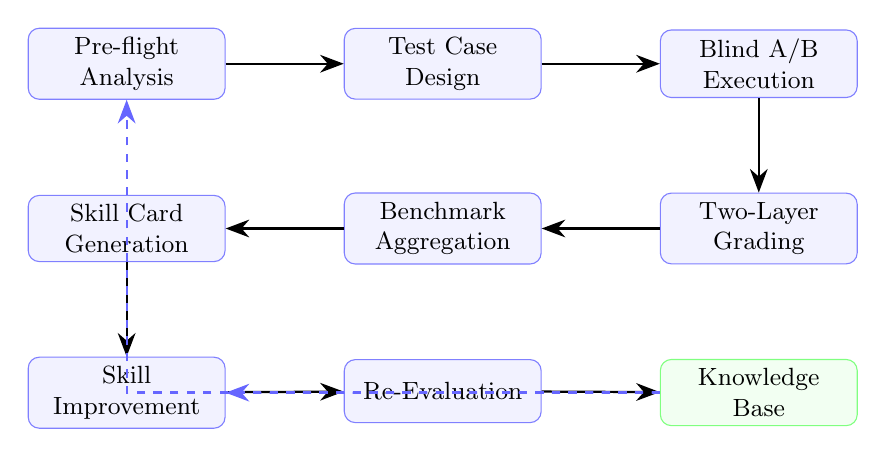
\begin{tikzpicture}[
    node distance=1.2cm and 1.5cm,
    box/.style={rectangle, draw=blue!50, fill=blue!5, rounded corners, minimum height=0.8cm, minimum width=2.5cm, align=center, font=\small},
    data/.style={rectangle, draw=green!50, fill=green!5, rounded corners, minimum height=0.8cm, minimum width=2.5cm, align=center, font=\small},
    arrow/.style={-{Stealth[length=3mm]}, thick}
]
\node[box] (preflight) {Pre-flight\\Analysis};
\node[box, right=of preflight] (design) {Test Case\\Design};
\node[box, right=of design] (exec) {Blind A/B\\Execution};
\node[box, below=of exec] (grade) {Two-Layer\\Grading};
\node[box, left=of grade] (bench) {Benchmark\\Aggregation};
\node[box, left=of bench] (card) {Skill Card\\Generation};
\node[data, below=of grade] (kb) {Knowledge\\Base};
\node[box, below=of card] (improve) {Skill\\Improvement};
\node[box, below=of bench] (reeval) {Re-Evaluation};

\draw[arrow] (preflight) -- (design);
\draw[arrow] (design) -- (exec);
\draw[arrow] (exec) -- (grade);
\draw[arrow] (grade) -- (bench);
\draw[arrow] (bench) -- (card);
\draw[arrow] (card) -- (improve);
\draw[arrow] (improve) -- (reeval);
\draw[arrow] (reeval) -- (kb);
\draw[arrow, dashed, blue!60] (kb) -| (preflight);
\draw[arrow, dashed, blue!60] (kb) -- (improve);
\end{tikzpicture}
\caption{PandaEval pipeline. Solid arrows show the evaluation flow; dashed arrows show the self-evolution feedback loop from the knowledge base back into pre-flight analysis and skill improvement.}
\label{fig:pipeline}
\end{figure}

The system produces the following artifacts per skill:

\begin{itemize}[leftmargin=*]
    \item \textbf{Eval config} (\texttt{evals/<slug>.json}): Test prompts and assertions
    \item \textbf{Workspace} (\texttt{workspaces/<slug>/}): Raw outputs from with-skill and without-skill runs, timing data, grading results
    \item \textbf{Skill card} (\texttt{skill-cards/<slug>-v<N>.md}): Standardized evaluation report modeled after HuggingFace model cards
    \item \textbf{Benchmark} (\texttt{benchmark.json}): Machine-readable aggregate statistics
\end{itemize}

Across 123 skills, this produced 150+ skill cards (including improvement comparison cards), an interactive HTML leaderboard, and executive reports in English and Chinese.

% ================================================================
\section{Limitations}
\label{sec:limitations}

\paragraph{Single execution model.}
All evaluations used Claude Opus 4. A skill that helps Claude may not help GPT-4.1 or Gemini. The v0.4.0 design supports cross-model evaluation but results are not yet available.

\paragraph{Same-model judging.}
Using the same model for execution and judging introduces potential self-grading bias. We prioritize deterministic (Layer 1) assertions to mitigate this, but rubric-based (Layer 2) assessments may be affected.

\paragraph{Test case coverage.}
Each skill was evaluated on 2--3 test cases. This is sufficient to detect major quality signals but may miss edge cases. Skills with many features or use cases are undersampled.

\paragraph{No real-user validation.}
All evaluations are automated. We have no human validation set confirming that PandaEval scores correlate with real user satisfaction. This is the most important gap.

\paragraph{Assertion design subjectivity.}
Test cases and assertions were designed by the evaluation engine (an LLM) based on each skill's \texttt{SKILL.md}. This means the evaluation is partially testing whether the skill's claims are internally consistent, not whether the skill meets external user needs.

\paragraph{Temporal snapshot.}
Evaluations reflect a single point in time. Skills and models evolve; scores may not hold as base models improve (potentially reducing the delta for capability-uplift skills).

% ================================================================
\section{Future Work}
\label{sec:future}

\paragraph{Cross-model evaluation.}
Deploy the v0.4.0 multi-model pipeline to test each skill across Claude, GPT-4.1, and Gemini, producing a model-skill compatibility matrix.

\paragraph{Human validation set.}
Recruit a panel of 20--50 ClawHub users to independently rate a subset of 30 skills. Compare human ratings against PandaEval scores to establish ground-truth correlation.

\paragraph{Cost-per-quality analysis.}
Normalize scores by dollar cost (tokens $\times$ model pricing) to answer: ``Is the quality improvement worth the extra spend?''

\paragraph{Longitudinal tracking.}
Re-evaluate the full corpus monthly to detect score drift as base models improve. This would reveal which skills remain valuable over time (encoded preferences) vs.\ which become redundant (capability uplift for now-known tools).

\paragraph{Skill composition.}
Test interactions between multiple active skills. Two individually-recommended skills may conflict or produce unexpected behavior when loaded simultaneously.

\paragraph{CI/CD integration.}
Enable skill authors to run PandaEval as a pre-publish quality gate, similar to running a test suite before merging code.

% ================================================================
\section{Conclusion}
\label{sec:conclusion}

We presented PandaEval, a self-evolving evaluation engine for AI agent skills, and applied it to 123 real skills from the ClawHub marketplace. Our core finding---that 76.4\% of skills measurably improve model output---provides the first empirical answer to the question of whether agent skills actually work.

But the more significant contribution is the self-evolving architecture itself. Static benchmarks measure a fixed set of capabilities at a point in time; PandaEval accumulates knowledge across evaluation batches and uses it to improve its own methodology. The evaluation engine evolved from 7~phases to 12~phases in five days, with each addition traceable to a specific empirical finding. The improvement engine went from ad hoc rewrites to a pattern library with tracked success rates after a single improvement cycle. Both loops are closed: evaluation knowledge flows back into evaluation methodology, and improvement knowledge flows back into improvement strategy selection.

This dual-loop self-evolution has a practical consequence: \textbf{the longer the system runs, the better it gets at both detecting and fixing skill quality issues}. A static benchmark would have caught the same 8 failure modes in its first pass and never improved. PandaEval discovered phantom tooling in Batch~3, added a pre-flight check in v0.3.0, and caught it systematically in all subsequent batches. The knowledge compounds.

The most actionable finding for skill authors remains concrete: \textbf{skills should be behavioral contracts, not textbooks}. Remove what the model already knows; add MUST/ALWAYS/NEVER rules for what should be different. The improvement pipeline proved this works: removing 60--80\% of content improved all three targeted skills by +1.5--2.0 points.

For the broader agent ecosystem, PandaEval suggests that quality assurance for AI agent skills is tractable and automatable---and that the systems doing the assurance should themselves be designed to learn and improve.

% ================================================================
\section*{Data Availability}

All evaluation artifacts, skill cards, the interactive leaderboard, and the evaluation engine methodology are publicly available at \url{https://github.com/SerendipityOneInc/PandaEval/}. 

% ================================================================
% References
\begin{thebibliography}{20}

\bibitem[Bradley and Terry(1952)]{bradley1952rank}
R.~A. Bradley and M.~E. Terry.
\newblock Rank analysis of incomplete block designs: I. The method of paired comparisons.
\newblock \emph{Biometrika}, 39(3/4):324--345, 1952.

\bibitem[Chen et~al.(2021)]{chen2021humaneval}
M.~Chen, J.~Tworek, H.~Jun, Q.~Yuan, H.~Pinto de~Oliveira, J.~Kaplan, H.~Edwards, Y.~Burda, N.~Joseph, G.~Brockman, et~al.
\newblock Evaluating large language models trained on code.
\newblock \emph{arXiv preprint arXiv:2107.03374}, 2021.

\bibitem[Chen et~al.(2023)]{chen2023teval}
Z.~Chen, W.~Du, W.~Zhang, K.~Liu, J.~Liu, M.~Lan, J.~Gong, and H.~Liu.
\newblock T-Eval: Evaluating the tool utilization capability step by step.
\newblock \emph{arXiv preprint arXiv:2312.14033}, 2023.

\bibitem[Chiang et~al.(2024)]{chiang2024chatbot}
W.-L. Chiang, L.~Zheng, Y.~Sheng, S.~Zhuang, Z.~Wu, Y.~Zhuang, Z.~Lin, Z.~Li, D.~Li, E.~P. Xing, H.~Zhang, J.~E. Gonzalez, and I.~Stoica.
\newblock Chatbot Arena: An open platform for evaluating LLMs by human preference.
\newblock \emph{arXiv preprint arXiv:2403.04132}, 2024.

\bibitem[Cobbe et~al.(2021)]{cobbe2021gsm8k}
K.~Cobbe, V.~Kosaraju, M.~Bavarian, M.~Chen, H.~Jun, L.~Kaiser, M.~Plappert, J.~Tworek, J.~Hilton, R.~Nakano, C.~Hesse, and J.~Schulman.
\newblock Training verifiers to solve math word problems.
\newblock \emph{arXiv preprint arXiv:2110.14168}, 2021.

\bibitem[Hendrycks et~al.(2021{\natexlab{a}})]{hendrycks2021mmlu}
D.~Hendrycks, C.~Burns, S.~Basart, A.~Zou, M.~Mazeika, D.~Song, and J.~Steinhardt.
\newblock Measuring massive multitask language understanding.
\newblock In \emph{ICLR}, 2021{\natexlab{a}}.

\bibitem[Hendrycks et~al.(2021{\natexlab{b}})]{hendrycks2021math}
D.~Hendrycks, C.~Burns, S.~Kadavath, A.~Arora, S.~Basart, E.~Tang, D.~Song, and J.~Steinhardt.
\newblock Measuring mathematical problem solving with the MATH dataset.
\newblock In \emph{NeurIPS}, 2021{\natexlab{b}}.

\bibitem[Hospedales et~al.(2022)]{hospedales2022metalearning}
T.~Hospedales, A.~Antoniou, P.~Micaelli, and A.~Storkey.
\newblock Meta-learning in neural networks: A survey.
\newblock \emph{IEEE TPAMI}, 44(9):5149--5169, 2022.

\bibitem[Huang et~al.(2023)]{huang2023selfimprove}
J.~Huang, S.~S. Gu, L.~Hou, Y.~Wu, X.~Wang, H.~Yu, and J.~Han.
\newblock Large language models can self-improve.
\newblock In \emph{EMNLP}, 2023.

\bibitem[Li et~al.(2023)]{li2023apibank}
M.~Li, Y.~Zhao, B.~Yu, F.~Song, H.~Li, H.~Yu, Z.~Li, F.~Huang, and Y.~Li.
\newblock API-Bank: A comprehensive benchmark for tool-augmented LLMs.
\newblock In \emph{EMNLP}, 2023.

\bibitem[Liu et~al.(2023)]{liu2023agentbench}
X.~Liu, H.~Yu, H.~Zhang, Y.~Xu, X.~Lei, H.~Lai, Y.~Gu, H.~Ding, K.~Men, K.~Yang, et~al.
\newblock AgentBench: Evaluating LLMs as agents.
\newblock In \emph{ICLR}, 2023.

\bibitem[Qin et~al.(2023)]{qin2023toolllm}
Y.~Qin, S.~Liang, Y.~Ye, K.~Zhu, L.~Yan, Y.~Lu, Y.~Lin, X.~Cong, X.~Tang, B.~Qian, et~al.
\newblock ToolLLM: Facilitating large language models to master 16000+ real-world APIs.
\newblock In \emph{ICLR}, 2023.

\bibitem[Schick et~al.(2023)]{schick2023toolformer}
T.~Schick, J.~Dwivedi-Yu, R.~Dess{\`i}, R.~Raileanu, M.~Lomeli, L.~Zettlemoyer, N.~Cancedda, and T.~Scialom.
\newblock Toolformer: Language models can teach themselves to use tools.
\newblock In \emph{NeurIPS}, 2023.

\bibitem[Shen et~al.(2023)]{shen2023taskbench}
Y.~Shen, K.~Song, X.~Tan, D.~Li, W.~Lu, and Y.~Zhuang.
\newblock TaskBench: Benchmarking large language models for task automation.
\newblock \emph{arXiv preprint arXiv:2311.18760}, 2023.

\bibitem[White et~al.(2024)]{white2024livebench}
C.~White, S.~Dooley, M.~Roberts, A.~Pal, B.~Feuer, S.~Jain, R.~Shwartz-Ziv, N.~Jain, K.~Saifullah, S.~Naber, et~al.
\newblock LiveBench: A challenging, contamination-free LLM benchmark.
\newblock \emph{arXiv preprint arXiv:2406.19314}, 2024.

\bibitem[Yao et~al.(2023)]{yao2023react}
S.~Yao, J.~Zhao, D.~Yu, N.~Du, I.~Shafran, K.~Narasimhan, and Y.~Cao.
\newblock ReAct: Synergizing reasoning and acting in language models.
\newblock In \emph{ICLR}, 2023.

\bibitem[Zheng et~al.(2023)]{zheng2023judging}
L.~Zheng, W.-L. Chiang, Y.~Sheng, S.~Zhuang, Z.~Wu, Y.~Zhuang, Z.~Lin, Z.~Li, D.~Li, E.~P. Xing, H.~Zhang, J.~E. Gonzalez, and I.~Stoica.
\newblock Judging LLM-as-a-judge with MT-Bench and Chatbot Arena.
\newblock In \emph{NeurIPS}, 2023.

\end{thebibliography}

\end{document}
